\section*{Math 202a - HW4 - Dan Davison - \texttt{ddavison@berkeley.edu}}
\begin{mdframed}
  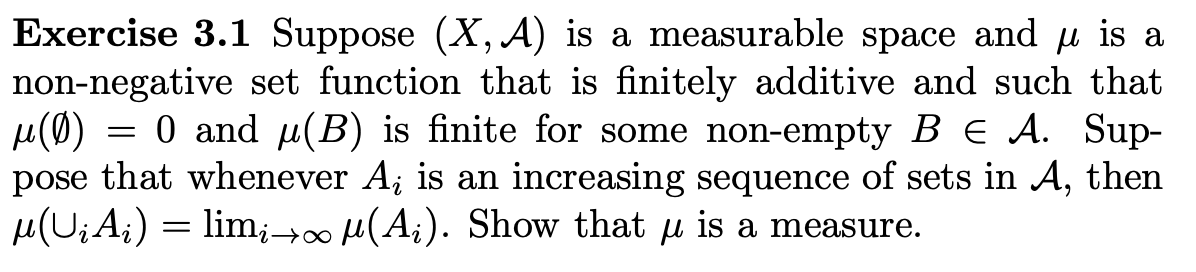
\includegraphics[width=400pt]{img/analysis--berkeley-202a-hw04-f604.png}
\end{mdframed}
\begin{claim*}
  $\mu$ is a measure.
\end{claim*}
\begin{proof}
  It is given that $\mu$ is non-negative and that $\mu(\emptyset) = 0$. We must prove that $\mu$ is countably
  additive.

  So let $B_1, B_2, \dots$ be a disjoint collection of subsets of $X$. We want to show
  that $\mu(\bigcup_{i=1}^\infty B_i) = \sum_{i=1}^\infty \mu(B_i)$.

  Let's construct an increasing sequence of sets. Define $A_j = \bigcup_{i \leq j} B_i$ for $j=1, 2, \dots$, so
  that $A_1, A_2, \dots$ is an increasing sequence of sets. Note
  that $\bigcup_{i=1}^\infty B_i = \bigcup_{j=1}^\infty A_j$ therefore, by
  hypothesis,
  $\mu\big(\bigcup_{i=1}^\infty B_i\big) = \mu\big(\bigcup_{j=1}^\infty A_j\big) = \lim_{j\to\infty} \mu(A_j)$.

  Now, from finite additivity we have
  \begin{align*}
    \mu(A_j) = \mu(\bigcup_{i \leq j} B_i) = \sum_{i\leq j} \mu(B_i),
  \end{align*}
  therefore
  \begin{align*}
    \mu\big(\bigcup_{i=1}^\infty B_i\big) = \lim_{j\to\infty} \sum_{i\leq j} \mu(B_i) = \sum_{i=1}^\infty \mu(B_i),
  \end{align*}
  as required.
\end{proof}

\newpage
\begin{mdframed}
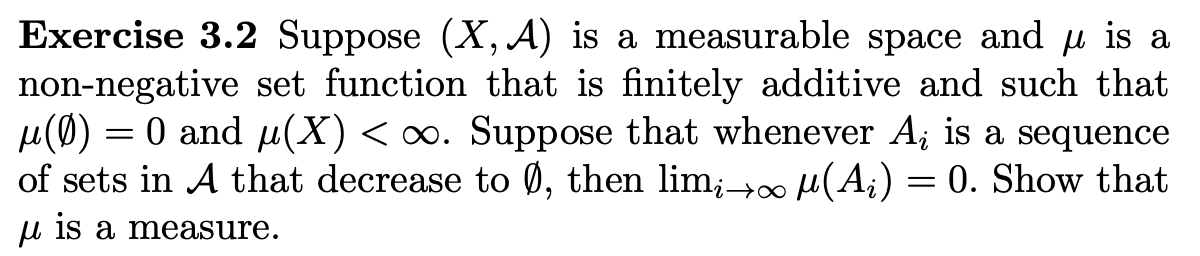
\includegraphics[width=400pt]{img/analysis--berkeley-202a-hw04-c187.png}
\end{mdframed}



\newpage
\begin{mdframed}
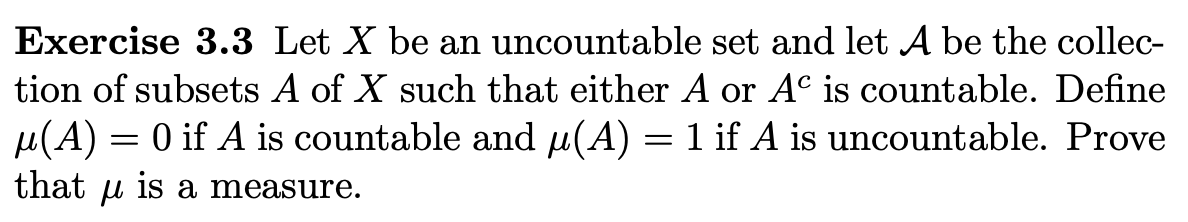
\includegraphics[width=400pt]{img/analysis--berkeley-202a-hw04-b168.png}
\end{mdframed}
\begin{proof}
  $\emptyset$ is countable, therefore we have $\mu(\emptyset) = 0$ as required, and it remains to show
  that $\mu$ is countably additive.

  So let $B_1, B_2, \dots$ be a disjoint countable collection of subsets of $X$. We want to show
  that $\mu(\bigcup_{i=1}^\infty B_i) = \sum_{i=1}^\infty \mu(B_i)$.

  % Consider $\bigcup_{i=1}^\infty B_i$. It could be uncountable, since the $B_i$ could be a countable partition
  % of the entire set $X$. Could it also be countable? Yes, since the $B_i$ could be singletons. So we must
  % handle both cases.

  First suppose $\bigcup_{i=1}^\infty B_i$ is countable. Then no $B_i$ is uncountable. Therefore $\mu(B_i) = 0$
  for all $i$ and we have
  \begin{align*}
    \sum_{i=1}^\infty \mu(B_i) = \sum_{i=1}^\infty 0 = 0 = \mu\big(\bigcup_{i=1}^\infty B_i\big),
  \end{align*}
  as required.

  Next, suppose $\bigcup_{i=1}^\infty B_i$ is uncountable. We want to show
  that $\sum_{i=1}^\infty \mu(B_i) = 1$. Equivalently, we want to show that exactly one of the $B_i$ is
  uncountable. Note that $\ms A = \sigma(\ms A)$, and therefore we have by hypothesis that either $B_i$ is
  countable or $B_i^c$ is countable, for all $i$. Clearly some $B_i$ is uncountable or else we would
  have $\sum_{i=1}^\infty \mu(B_i) = \sum_{i=1}^\infty 0 = 0 \neq \mu\big(\bigcup_{i=1}^\infty B_i\big)$.
  Suppose for a contradiction that there exists $j \neq k$ such that $B_j$ and $B_k$ are uncountable. Note
  that $B_j$ and $B_k$ are disjoint, therefore $B_k \subseteq B_j^c$. But $B_j^c$ is countable, therefore $B_k$
  is countable; a contradiction. Therefore no such pair $j, k$ exists and we conclude that exactly one of
  the $B_i$ is uncountable, as required.
\end{proof}

\newpage
\begin{mdframed}
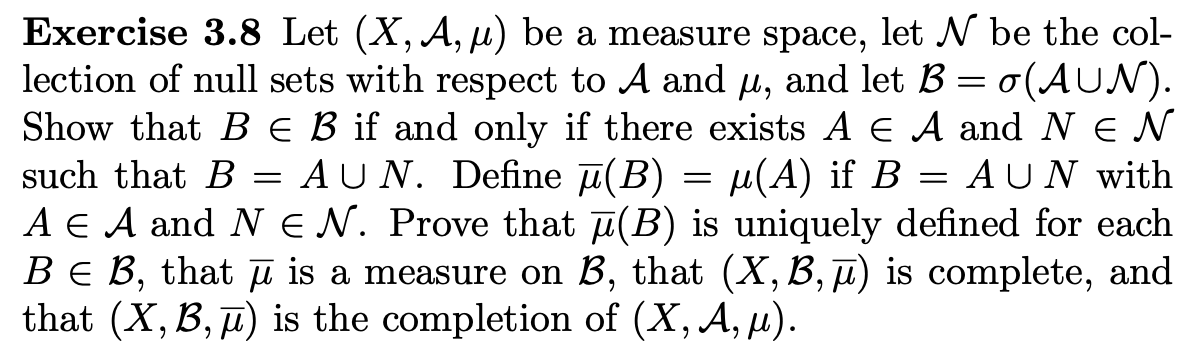
\includegraphics[width=400pt]{img/analysis--berkeley-202a-hw04-c88b.png}
\end{mdframed}

\newpage
\begin{mdframed}
  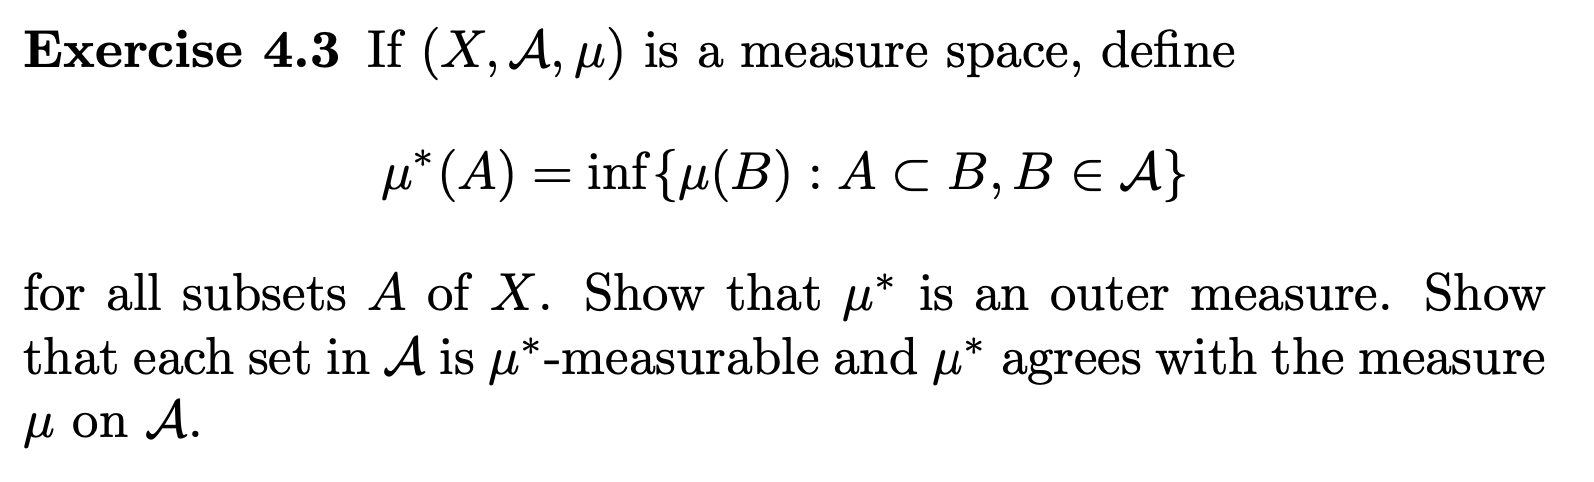
\includegraphics[width=400pt]{img/analysis--berkeley-202a-hw-0d98.png}
\end{mdframed}


\newpage
\begin{mdframed}
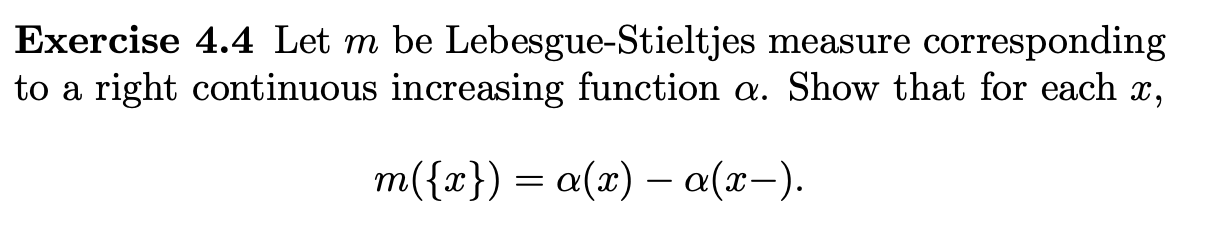
\includegraphics[width=400pt]{img/analysis--berkeley-202a-hw04-c0b6.png}
\end{mdframed}

\newpage


\begin{comment}
  EXERCISE 3.3 FROM OLD VERSION
  \begin{mdframed}
    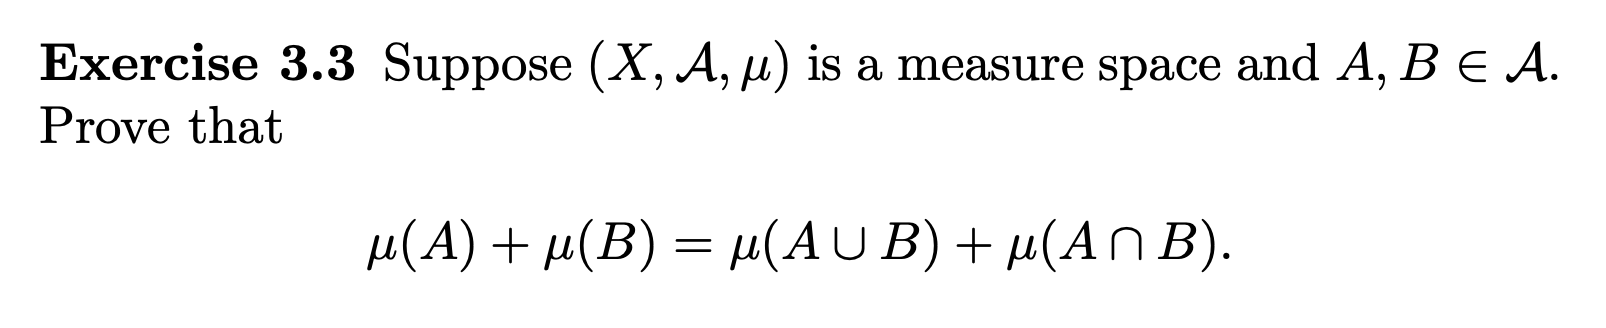
\includegraphics[width=400pt]{img/analysis--berkeley-202a-hw-2389.png}
  \end{mdframed}

  \begin{proof}
    From finite additivity we have
    \begin{align*}
      \mu(A \cup B) &= \mu(A) + \mu(A \setminus B). \\
      \mu(A \cup B) &= \mu(B) + \mu(B \setminus A).
    \end{align*}
    Summing these gives
    \begin{align*}
      2\mu(A \cup B)
      = \mu(A) + \mu(B) + \mu(A \triangle B)
    \end{align*}
    But $\{A \triangle B, A \cap B\}$ is a partition of $A \cup B$ hence from finite additivity
    again $\mu(A \triangle B) + \mu(A \cap B) = \mu(A \cup B)$. Therefore
    \begin{align*}
      2\mu(A \cup B) = \mu(A) + \mu(B) + \mu(A \cup B) - \mu(A \cap B),
    \end{align*}
    or equivalently
    \begin{align*}
      \mu(A \cup B) = \mu(A) + \mu(B) - \mu(A \cap B).
    \end{align*}
  \end{proof}

  \begin{mdframed}
    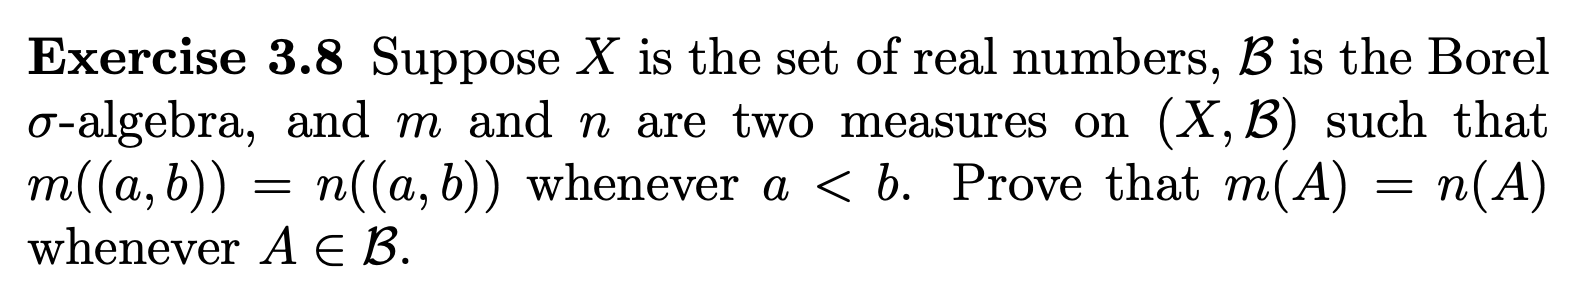
\includegraphics[width=400pt]{img/analysis--berkeley-202a-hw-3a79.png}
  \end{mdframed}

  \begin{claim*}
    If $m$ and $n$ have the same value on any open interval in $B$ then they have the same value on any set
    in $\mc B$.
  \end{claim*}

  \begin{proof}
    Let $\mc O$ be the collection of open subsets of $\R$.

    Let $O \in \mc O$. Then $O$ can be written as a countable union of disjoint open intervals, $O = \bigcup_i I_i$. Therefore
    \begin{align*}
      m(O) = m(\bigcup_i I_i) = \sum_i m(I_i) = \sum_i n(I_i) = n(O).
    \end{align*}
    By definition, $\mc B = \sigma(\mc O)$. We want to show that measures $m$ and $n$ agree on every set $A \in \mc B$.

    Let $A \in \mc B$ and suppose $m(A) = n(A)$. Then
    \begin{align*}
      m(A^c) = m(X) - m(A) = n(X) - n(A) = n(A^c).
    \end{align*}
  \end{proof}
\end{comment}
